\section{Repeated Measures ANOVA}
\begin{frame}\frametitle{Repeated Measures ANOVA (rma)}
  \begin{itemize}
  \item equivalent of the one-way ANOVA, but for related, not independent groups,  \item in that sense it is the extension of the dependent t-test: he same people are being measured more than once on the same dependent variable
  \item here we will look at the simplest design of rma
  \end{itemize}
\end{frame}


\begin{frame}\frametitle{Statistical Model}
  \begin{itemize}
  \item remember in basic one-way Anova $$Y_{ij} = \mu + \alpha_j + Error_{ij}$$
  \item error was assumed to have variance of $\sigma^2_{error}$
  \item measurements and therefore the errors were independed
  \end{itemize}
\end{frame}


\begin{frame}\frametitle{Statistical Model}
  \begin{itemize}
  \item in repeated measurement Anova $$Y_{ij} = \mu + time_j + S_j + (time\times S)_{ij} + Error_{ij}$$
  \item assumes still thant errors have the same variances and
  \item covariances are the same
  \end{itemize}
\end{frame}



\begin{frame}\frametitle{Repeated Measures ANOVA (rma)}
  \begin{itemize}
  \item main hypothesis of rma: $$\mu_1=\mu_2=\ldots =\mu_n$$
  \item here we will look at the simplest design of rma
  \item in this design the within group variance from above is splitted in variance caused by subject variability and the error variance (where in the anova from above we had only error) 
  \end{itemize}
\end{frame}


\begin{frame}\frametitle{Repeated Measures ANOVA (rma)}
So we have one more sum of sqares:
  \begin{itemize}
  \item $SS_{Time}$
  \item $SS_{within}$
  \item $SS_{Subject}$
  \item $SS_{error}$
  \end{itemize}
\end{frame}

\begin{frame}[fragile, allowframebreaks]\frametitle{Example}\scriptsize
\begin{verbatim}
> xx
  subject t1 t2 t3
1       1 45 50 55
2       2 42 42 45
3       3 36 41 43
4       4 39 35 40
5       5 51 55 59
6       6 44 49 56
> n <- 6
> k <- 3
> require(reshape2)
> xx <- melt(xx,id.vars = "subject")  
> ## Sum of Squares time
> (tmp <- aggregate(value ~ variable,FUN = "mean",data=xx))
  variable    value
1       t1 42.83333
2       t2 45.33333
3       t3 49.66667
> (sstime <- sum(6*(tmp$value - mean(xx$value))**2))
[1] 143.4444
> ## sum of squares within
> (xx <- xx %>% group_by(variable) %>% mutate(gr.mean=mean(value)))
Source: local data frame [18 x 4]
Groups: variable

   subject variable value  gr.mean
1        1       t1    45 42.83333
2        2       t1    42 42.83333
3        3       t1    36 42.83333
4        4       t1    39 42.83333
5        5       t1    51 42.83333
6        6       t1    44 42.83333
7        1       t2    50 45.33333
8        2       t2    42 45.33333
9        3       t2    41 45.33333
10       4       t2    35 45.33333
11       5       t2    55 45.33333
12       6       t2    49 45.33333
13       1       t3    55 49.66667
14       2       t3    45 49.66667
15       3       t3    43 49.66667
16       4       t3    40 49.66667
17       5       t3    59 49.66667
18       6       t3    56 49.66667
> (ssw <- sum((xx$value - xx$gr.mean)**2))
[1] 715.5
> ## sum of squares sub
> (sub.xx <- xx %>% group_by(subject) %>% summarise(sub.mean=mean(value)))
Source: local data frame [6 x 2]

  subject sub.mean
1       1 50.00000
2       2 43.00000
3       3 40.00000
4       4 38.00000
5       5 55.00000
6       6 49.66667
> (sssub <- k*sum((sub.xx$sub.mean - mean(xx$value))**2))
[1] 658.2778
> ## sum of squares error
> (sserror <- ssw - sssub)
[1] 57.22222
> ## ssw
\end{verbatim}
\end{frame}


\begin{frame}[fragile, allowframebreaks]\frametitle{Example}
  \begin{itemize}
  \item now it is ease to calculate the meas squares and the F statistic
  \end{itemize}\scriptsize
\begin{verbatim}
> ## mean squares
> (mstime <- sstime/(k-1))
[1] 71.72222
> (mserror <- sserror/((n-1)*(k-1)))
[1] 5.722222
> (F <- mstime/mserror)
[1] 12.53398
> pf(F,k-1,((n-1)*(k-1)))
[1] 0.9981144
> 1-pf(F,k-1,((n-1)*(k-1)))
[1] 0.001885591
\end{verbatim}
\end{frame}

\begin{frame}[fragile, allowframebreaks]\frametitle{Example}\scriptsize
\begin{verbatim}
> require(ez)
> xx <- as.data.frame(xx)
> (an <- ezANOVA(data=xx,dv = value,wid= subject, within = variable))
Warnung: Converting "subject" to factor for ANOVA.
$ANOVA
    Effect DFn DFd        F           p p<.05       ges
2 variable   2  10 12.53398 0.001885591     * 0.1670008

$`Mauchly's Test for Sphericity`
    Effect         W         p p<.05
2 variable 0.4335338 0.1879515      

$`Sphericity Corrections`
    Effect       GGe       p[GG] p[GG]<.05      HFe       p[HF] p[HF]<.05
2 variable 0.6383796 0.008985215         * 0.760165 0.005284458         *
\end{verbatim}
\end{frame}


\section{Multivariate Analysis of Variance}
\begin{frame}\frametitle{MANOVA}
  \begin{itemize}
  \item in general, the framework of multivariate linear models extends quite elegantly to repeated-measure design
  \item the $p$ responses per individual related to the dependend variables in the model
  \item the treatment sum of squares and the error sum of squares from the univariate case last week extends to the $p \times p$ sum of squares and crossproducts
$$ \mathbb{H}\equiv \mathbb{SSP_{H}}$$ and $$ \mathbb{E}\equiv \mathbb{SSP_{E}}$$
  \item test statistics (Wilks $\Lambda$, Pillai trace, Hotelling-Lawley trace, Roys maximum root) for testing are based on the non-zero latent roots of $\mathbb{HE^{-1}}$ and attempt to capture how large $\mathbb{H}$ relative to $\mathbb{E}$
  \item all these statistics have transformations to F 
  \end{itemize}
\end{frame}

\begin{frame}\frametitle{Example Data}
  \begin{itemize}
  \item weights of guinea pigs under three levels of vitamin E supplements
  \item measured six times at the end of week 1, 3, 4, 5, 6, and 7
  \item contained in guinea.rdata
  \item Crowder and Hand 1990
  \end{itemize}
\end{frame}


\begin{frame}[fragile]\frametitle{Example Data}
  \begin{itemize}
  \item load the data print them on the screen \scriptsize
\begin{verbatim}
> load("guinea.rdata")
> head(guinea,10)
   Dose Animal  X1  X3  X4  X5  X6  X7
1     0      1 455 460 510 504 436 466
2     0      2 467 565 610 596 542 587
3     0      3 445 530 580 597 582 619
4     0      4 485 542 594 583 611 612
5     0      5 480 500 550 528 562 576
6     1      6 514 560 565 524 552 597
7     1      7 440 480 536 484 567 569
8     1      8 495 570 569 585 576 677
9     1      9 520 590 610 637 671 702
10    1     10 503 555 591 605 649 675
\end{verbatim}
  \end{itemize}
\end{frame}


\begin{frame}[fragile]\frametitle{Example Data}
  \begin{itemize}
  \item reshape the data for ggplot2
  \item plot boxplots and means per treatment group \scriptsize
\begin{verbatim}
> require(reshape2)
> dl <- melt(guinea,id.vars = c("Dose","Animal"))
> dl$variable <- extract_numeric(dl$variable)
> dl$group <- factor(dl$Dose)
> head(dl)
  Dose Animal variable value group
1    0      1        1   455     0
2    0      2        1   467     0
3    0      3        1   445     0
4    0      4        1   485     0
5    0      5        1   480     0
6    1      6        1   514     1
\end{verbatim}
  \end{itemize}
\end{frame}

\begin{frame}[fragile]\frametitle{Example Data}
\scriptsize
\begin{verbatim}
> ggplot(dl,aes(x=variable,y=value,colour=group)) +
+     geom_boxplot(aes(x=variable,group=factor(variable))) +
+     stat_summary(fun.y="mean",geom = "line") 
\end{verbatim}
  \begin{center}
    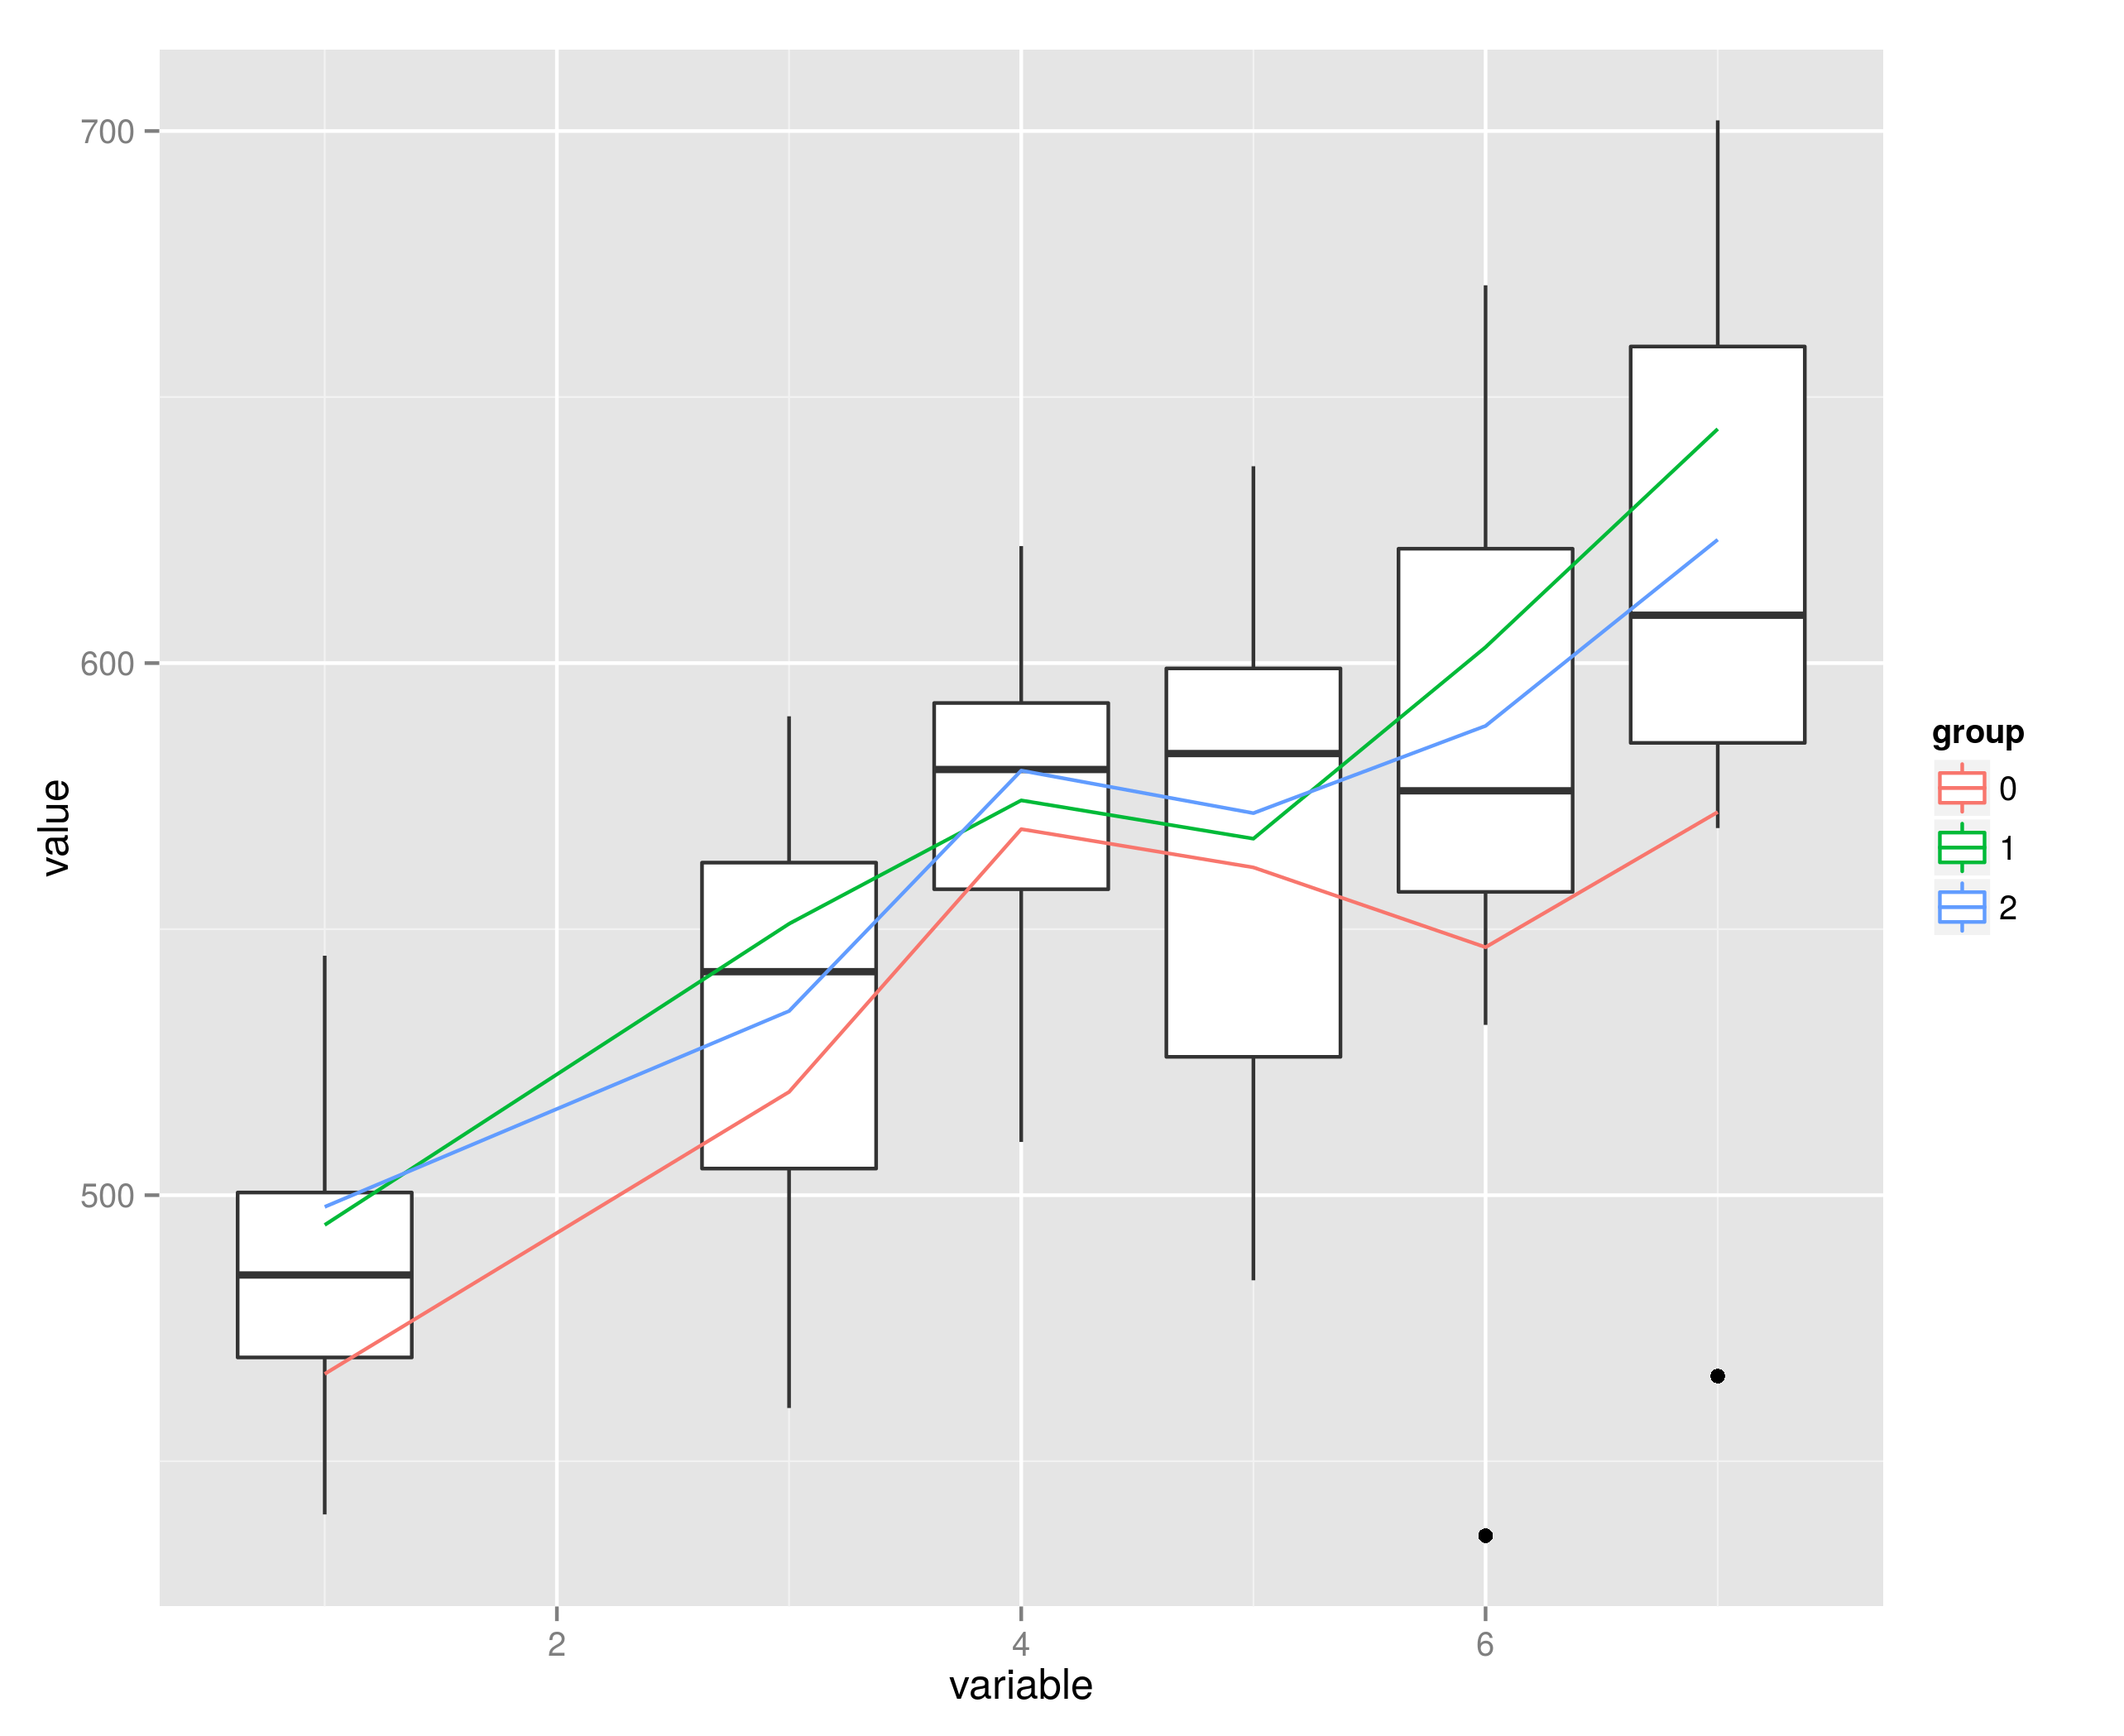
\includegraphics[width=11cm, height=7cm]{rma1.png}
  \end{center}
\end{frame}

\begin{frame}[fragile]\frametitle{Basic multivariate model}
  \begin{itemize}
  \item basic MVLM with an intercept only
  \item intercepts estimate the means at each instant of time
  \end{itemize}\scriptsize
\begin{verbatim}
> ## model
> guinea$Dosef <- factor(guinea$Dose)
> ### Basic multivariate linear model
> mod <- lm(cbind(X1,X3,X4,X5,X6,X7) ~ 1,data=guinea)
> (mod <- lm(cbind(X1,X3,X4,X5,X6,X7) ~ 1,data=guinea))

Call:
lm(formula = cbind(X1, X3, X4, X5, X6, X7) ~ 1, data = guinea)

Coefficients:
             X1     X3     X4     X5     X6     X7   
(Intercept)  486.2  535.0  574.3  566.8  579.3  613.1
\end{verbatim}
\end{frame}


\begin{frame}[fragile]\frametitle{Basic multivariate model}
  \begin{itemize}
  \item now test the Null hypothesis $$\mu_1=\mu_2=\ldots =\mu_n$$
  \item it is the simplest case of a multivariate test
  \end{itemize}\scriptsize
\begin{verbatim}
> (av <- Anova(mod))
Note: model has only an intercept; equivalent type-III tests substituted.

Type III MANOVA Tests: Pillai test statistic
            Df test stat approx F num Df den Df    Pr(>F)    
(Intercept)  1   0.99888   1341.3      6      9 9.286e-13 ***
---
Signif. codes:  0 ‘***’ 0.001 ‘**’ 0.01 ‘*’ 0.05 ‘.’ 0.1 ‘ ’ 1
\end{verbatim}
\end{frame}

\begin{frame}[fragile]\frametitle{Extract $\mathbb{H}$}
  \begin{itemize}
  \item extract the sum of squares and products matrix a) for hypothesis
  \end{itemize}\scriptsize
\begin{verbatim}
> av$SSP
$`(Intercept)`
        X1      X3      X4      X5      X6      X7
X1 3545857 3901755 4188127 4133672 4224592 4471095
X3 3901755 4293375 4608490 4548570 4648615 4919860
X4 4188127 4608490 4946733 4882415 4989803 5280956
X5 4133672 4548570 4882415 4818934 4924925 5212293
X6 4224592 4648615 4989803 4924925 5033248 5326936
X7 4471095 4919860 5280956 5212293 5326936 5637761  
\end{verbatim}
\end{frame}


\begin{frame}[fragile]\frametitle{Extract $\mathbb{E}$}
  \begin{itemize}
  \item extract the sum of squares and products matrix b) for errors
  \end{itemize}\scriptsize
\begin{verbatim}
> av$SSPE
        X1    X3       X4      X5       X6       X7
X1 11450.4 10716  5679.20  9326.6 13435.20 14389.80
X3 10716.0 19668 13703.00 19888.0 21463.00 25693.00
X4  5679.2 13703 13294.93 17357.8 18419.93 19089.73
X5  9326.6 19888 17357.80 29166.4 27322.80 29977.20
X6 13435.2 21463 18419.93 27322.8 45448.93 42336.73
X7 14389.8 25693 19089.73 29977.2 42336.73 47268.93
\end{verbatim}
\end{frame}


\begin{frame}[fragile]\frametitle{HE plot}
  \begin{itemize}
  \item  size of the (degenerate) ellipse for the intercept term relative to that for Error gives the strength of evidence for the difference between the sample means and the means under
  \item the $\mathbb{H}$ ellipse extends outside the $\mathbb{E}$ ellipse (anywhere), this signals that $H_0$ is clearly rejected (for some linear combination of the response variables)
  \end{itemize}
  \begin{center}
    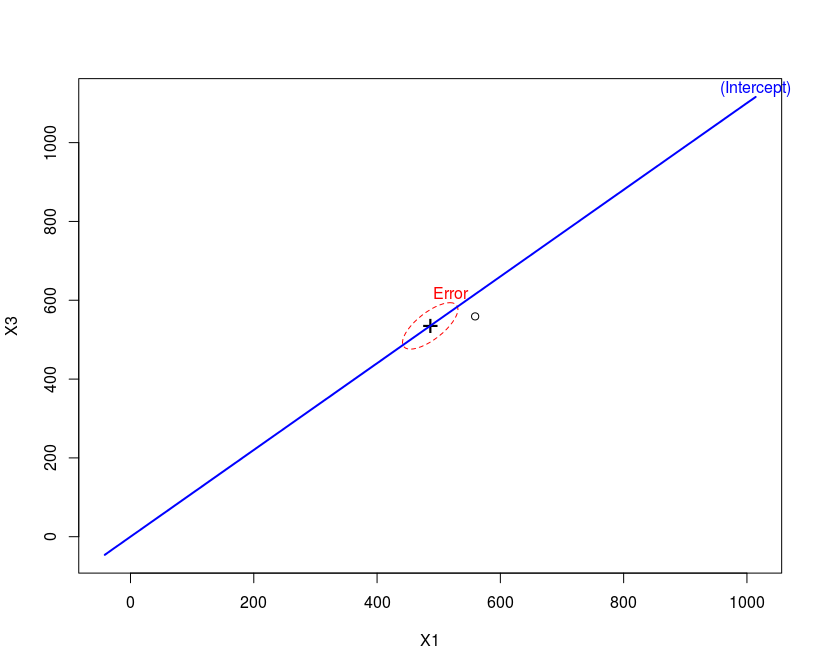
\includegraphics[height=5cm]{rma2.png}
  \end{center}
\end{frame}

\begin{frame}[fragile]\frametitle{Testing within-S effects}
  \begin{itemize}
  \item for repeated measurement design we need to specify the intra-subject design
  \item  structure  for  within-S  effects is specified through the arguments \texttt{idata} and \texttt{idesign}
  \item we need to contruct a time variable for the different measurement times
  \end{itemize}\scriptsize
\begin{verbatim}
> idata <- data.frame(time=factor(c(1,3:7)))
> (av2 <- Anova(mod, idata = idata, idesign = ~time))
Note: model has only an intercept; equivalent type-III tests substituted.

Type III Repeated Measures MANOVA Tests: Pillai test statistic
            Df test stat approx F num Df den Df    Pr(>F)    
(Intercept)  1   0.99561   3176.8      1     14 < 2.2e-16 ***
time         1   0.95566     43.1      5     10 1.899e-06 ***
---
Signif. codes:  0 ‘***’ 0.001 ‘**’ 0.01 ‘*’ 0.05 ‘.’ 0.1 ‘ ’ 1  
\end{verbatim}
\end{frame}

\begin{frame}[fragile,allowframebreaks]\frametitle{Add between-S effects}
  \begin{itemize}
  \item now add the group term to the model (Dosef)
  \end{itemize}\tiny
\begin{verbatim}
> (mod2 <- lm(cbind(X1,X3,X4,X5,X6,X7) ~ Dosef,data=guinea))

Call:
lm(formula = cbind(X1, X3, X4, X5, X6, X7) ~ Dosef, data = guinea)

Coefficients:
             X1     X3     X4     X5     X6     X7   
(Intercept)  466.4  519.4  568.8  561.6  546.6  572.0
Dosef1        28.0   31.6    5.4    5.4   56.4   72.0
Dosef2        31.4   15.2   11.0   10.2   41.6   51.2

> idata <- data.frame(time)
> (av2.mod2 <- Anova(mod2, idata = idata, idesign = ~time))

Type II Repeated Measures MANOVA Tests: Pillai test statistic
            Df test stat approx F num Df den Df    Pr(>F)    
(Intercept)  1   0.99627   3202.0      1     12 6.121e-16 ***
Dosef        2   0.14960      1.1      2     12   0.37821    
time         1   0.96118     39.6      5      8 1.954e-05 ***
Dosef:time   2   1.07059      2.1     10     18   0.08557 .  
---
Signif. codes:  0 ‘***’ 0.001 ‘**’ 0.01 ‘*’ 0.05 ‘.’ 0.1 ‘ ’ 1
\end{verbatim}
\end{frame}

\begin{frame}[allowframebreaks]\frametitle{Assumptions MANOVA}
  \begin{itemize}
  \item Normal Distribution: The dependent variable should be normally distributed within groups.  Overall, the F test is robust to non-normality, if the non-normality is caused by skewness rather than by outliers.
  \item Linearity: MANOVA assumes that there are linear relationships among all pairs of dependent variables, all pairs of covariates, and all dependent variable-covariate pairs in each cell.  Therefore, when the relationship deviates from linearity, the power of the analysis will be compromised.
  \item Remember that the error variance is computed (SS error) by adding up the sums of squares within each group. If the variances in the two groups are different from each other, then adding the two together is not appropriate, and will not yield an estimate of the common within-group variance.  Homoscedasticity can be examined graphically or by means of a number of statistical tests.
  \item Homogeneity of Variances and Covariances: In multivariate designs, with multiple dependent measures, the homogeneity of variances assumption described earlier also applies. However, since there are multiple dependent variables, it is also required that their intercorrelations (covariances) are homogeneous across the cells of the design. There are various specific tests of this assumption.
  \item Outliers: Like ANOVA, MANOVA is extremely sensitive to outliers.  Outliers may produce either a Type I or Type II error and give no indication as to which type of error is occurring in the analysis.  There are several programs available to test for univariate and multivariate outliers.
  \item Multicollinearity and Singularity: When there is high correlation between dependent variables, one dependent variable becomes a near-linear combination of the other dependent variables.  Under such circumstances, it would become statistically redundant and suspect to include both combinations.
  \end{itemize}

\end{frame}

\section{Mixed Models}
\begin{frame}[fragile, allowframebreaks]\frametitle{Alternative Approach - Mixed Model}
  \begin{itemize}
  \item the mixed model looks very similar to ANOVA: $$Y_{ij} = \mu + \alpha_j + S_i + Error_{ij}$$
  \item the difference is the assumption:
    \begin{itemize}
    \item $\mu$ is a fixed effect: no estimate of variability
    \item $\alpha_j$ are also fixed effects: no estimate of variability
    \item $S_i$ are random effects have normal distribution with zero mean
    \item $E_{ij}$ are normally distributed with mean zero (as usual)
    \end{itemize}
  \end{itemize}\scriptsize
\begin{verbatim}
> dl$variable <- factor(dl$variable)
> require(nlme)
> Lme.mod <- lme(value ~ group * variable, random = ~ 1 | Animal, data = dl)
> anova(Lme.mod)
               numDF denDF  F-value p-value
(Intercept)        1    60 3201.999  <.0001
group              2    12    1.056  0.3782
variable           5    60   52.550  <.0001
group:variable    10    60    1.799  0.0801
\end{verbatim}
\end{frame}

\begin{frame}[fragile, allowframebreaks]\frametitle{Alternative Approach - Mixed Model}
  \scriptsize
\begin{verbatim}
> require(lme4)
> Lme.mod <- lmer(value ~ group * variable + (1 | Animal), data = dl)
> anova(Lme.mod)
Analysis of Variance Table
               Df Sum Sq Mean Sq F value
group           2   1145   572.7  1.0555
variable        5 142554 28510.9 52.5505
group:variable 10   9763   976.3  1.7994
> fixed.effects(Lme.mod)
     (Intercept)           group1           group2        variable3 
           466.4             28.0             31.4             53.0 
       variable4        variable5        variable6        variable7 
           102.4             95.2             80.2            105.6 
group1:variable3 group2:variable3 group1:variable4 group2:variable4 
             3.6            -16.2            -22.6            -20.4 
group1:variable5 group2:variable5 group1:variable6 group2:variable6 
           -22.6            -21.2             28.4             10.2 
group1:variable7 group2:variable7 
            44.0             19.8 
\end{verbatim}
\end{frame}


\begin{frame}[fragile, allowframebreaks]\frametitle{Alternative Approach - Mixed Model}
  \begin{itemize}
  \item extract fixed effects
  \end{itemize}
  \scriptsize
\begin{verbatim}
> fixed.effects(Lme.mod)
     (Intercept)           group1           group2        variable3 
           466.4             28.0             31.4             53.0 
       variable4        variable5        variable6        variable7 
           102.4             95.2             80.2            105.6 
group1:variable3 group2:variable3 group1:variable4 group2:variable4 
             3.6            -16.2            -22.6            -20.4 
group1:variable5 group2:variable5 group1:variable6 group2:variable6 
           -22.6            -21.2             28.4             10.2 
group1:variable7 group2:variable7 
            44.0             19.8 
\end{verbatim}
\end{frame}

\begin{frame}[fragile, allowframebreaks]\frametitle{Alternative Approach - Mixed Model}
  \begin{itemize}
  \item post hoc test
  \end{itemize}
  \scriptsize
\begin{verbatim}
> summary(glht(Lme.mod, linfct=mcp(group="Tukey")))

	 Simultaneous Tests for General Linear Hypotheses

Multiple Comparisons of Means: Tukey Contrasts


Fit: lmer(formula = value ~ group * variable + (1 | Animal), data = dl)

Linear Hypotheses:
           Estimate Std. Error z value Pr(>|z|)
1 - 0 == 0    28.00      27.69   1.011    0.570
2 - 0 == 0    31.40      27.69   1.134    0.493
2 - 1 == 0     3.40      27.69   0.123    0.992
(Adjusted p values reported -- single-step method)

Warnmeldung:
In mcp2matrix(model, linfct = linfct) :
  covariate interactions found -- default contrast might be inappropriate
\end{verbatim}
\end{frame}

\begin{frame}[fragile,allowframebreaks]\frametitle{Mixed Models}
  \begin{itemize}
  \item average the interaction term
  \end{itemize}
\scriptsize
\begin{verbatim}
> ## consider interaction terms
> summary(glht(Lme.mod, linfct=mcp(group="Tukey",interaction_average = TRUE)))

	 Simultaneous Tests for General Linear Hypotheses

Multiple Comparisons of Means: Tukey Contrasts


Fit: lmer(formula = value ~ group * variable + (1 | Animal), data = dl)

Linear Hypotheses:
           Estimate Std. Error z value Pr(>|z|)
1 - 0 == 0   33.133     24.202   1.369    0.357
2 - 0 == 0   26.767     24.202   1.106    0.510
2 - 1 == 0   -6.367     24.202  -0.263    0.963
(Adjusted p values reported -- single-step method)
\end{verbatim}
\end{frame}


\begin{frame}[fragile,allowframebreaks]\frametitle{Mixed Models}
\scriptsize
\begin{verbatim}
  > Lme.mod <- lmer(value ~ group + variable + (1 | Animal), data = dl)
  > anova(Lme.mod)
  Analysis of Variance Table
  Df Sum Sq Mean Sq F value
  group     2   1276   638.1  1.0555
  variable  5 142555 28510.9 47.1641
  > summary(glht(Lme.mod, linfct=mcp(group="Tukey")))

  Simultaneous Tests for General Linear Hypotheses

  Multiple Comparisons of Means: Tukey Contrasts


  Fit: lmer(formula = value ~ group + variable + (1 | Animal), data = dl)

  Linear Hypotheses:
  Estimate Std. Error z value Pr(>|z|)
  1 - 0 == 0   33.133     24.202   1.369    0.357
  2 - 0 == 0   26.767     24.202   1.106    0.510
  2 - 1 == 0   -6.367     24.202  -0.263    0.963
  (Adjusted p values reported -- single-step method)
\end{verbatim}
\end{frame}



